\documentclass{article}

\usepackage{geometry}
\geometry{a4paper}
\setlength{\parindent}{10mm}
\setlength{\parskip}{0.9em}
\def\baselinestretch{1.5}

\usepackage[spanish]{babel}
%\renewcommand {\spanishtablename}{Tabla}
\usepackage[spanish,onelanguage,ruled]{algorithm2e}
\usepackage[utf8]{inputenc}
\usepackage{graphicx}
\usepackage{caption} 
\usepackage{amsmath, amsthm, amsfonts}
\usepackage{enumerate} 
\usepackage{fancyhdr}
\usepackage{anysize} 
\usepackage[usenames]{color}
\usepackage{booktabs}
\usepackage{etoolbox}
 \usepackage{fancyvrb}
 \usepackage{color,soul}
 \usepackage[dvipsnames]{xcolor}
 \usepackage{graphicx}
\usepackage{subcaption}
\usepackage{listings}
 

\usepackage{verbatim}
% redefine \VerbatimInput
\RecustomVerbatimCommand{\VerbatimInput}{VerbatimInput}%
 {fontsize=\footnotesize,
  %
  frame=lines,  % top and bottom rule only
  framesep=1em, % separation between frame and text
  rulecolor=\color{Gray},
  %
  label=\fbox{\color{Black}test.txt},
  labelposition=topline,
  %
  %commandchars=\|\(\), % escape character and argument delimiters for
                  % commands within the verbatim
  %commentchar=*        % comment character
 }


\pagestyle{fancy}

\chead{}
\lhead{} 
\rhead{}
\lfoot{\it }
\cfoot{}
\rfoot{\thepage}

\title{
\centering
Modelos Probabilistas Aplicados \\
Johanna Bolaños Zúñiga \\
Matricula: 1883900\\
Tarea 6
}

\date{}

\begin{document}
\maketitle

\section{Pruebas estadísticas}

Para realizar algunas las pruebas estadísticas se utilizó la información del Índice Nacional de Precios al Consumidor (INPC)\footnote{El INPC es un indicador económico que muestra la variación de los precios en un periodo de tiempo.} mensual por ciudades en el periodo desde enero 2015 a agosto 2020. Esta información fue consultada en la página del INEGI \cite{INEGI}, en la sección de Precios. Se utilizó el programa R versión 4.0.2. \cite{r} basado en la información encontrada en \textit{Statistical Tests} \cite{test} para la ejecución de algunas de las pruebas.

La información de las $55$ ciudades del INPC y su respectivo índice con base en la segunda quincena de julio 2018, fueron descargadas en un archivo \texttt{xlsx}. Posteriormente, estos datos se guardaron en un archivo \texttt{txt} para su tratamiento en el programa R.

Para efectos del estudio, se determinaron dos conjuntos de muestras, el primer conjunto (Conjunto 1) consiste en contemplar solo la información de las $3$ principales ciudades de México (Monterrey, Ciudad de México y Guadalajara) por separado. En el segundo (Conjunto 2), se consideró la información de los índices de todas las ciudades en los meses de agosto 2018, julio 2019 y agosto 2020. En todas las pruebas para aceptar la $H_{0}$, el valor $p$ debe ser mayor a 0.05 (nivel de significancia $\alpha$).

\subsection{Prueba Shapiro\textendash Wilks}
Esta prueba plantea la hipótesis nula ($H_{0}$) de que los datos provienen de una distribución normal y una hipótesis alternativa ($H_{1}$) que sostiene que la distribución no es normal.

Se realizó esta prueba con la función \texttt{shapiro.test} para determinar, si los datos del Conjunto 1 y 2 siguen una distribución normal. En el cuadro \ref{shapiroC1C2}, se muestran los valores de $p$ obtenidos para los datos de estos conjuntos. En el cual podemos observar que en el Conjunto 1, el valor $p$ es menor a $0.05$ para cada ciudad analizada, por lo tanto, se rechaza la $H_{0}$ lo que significa que los datos analizados al parecer no siguen una distribución normal. 

No obstante, para el Conjunto 2, los datos de cada mes analizado suponen seguir una distribución normal (valor $p >$ 0.05), lo cual podemos observarlo también en la figura \ref{normalesC2}.
    
\begin{table}
\centering
\caption{Resultados de la prueba de Shapiro\textendash Wilks aplicada a los Conjuntos 1 y 2}
\begin{tabular}{|c|l|r|}
\hline
\textbf{Conjunto}  & \multicolumn{1}{c|}{\textbf{Contenido}} & \multicolumn{1}{c|}{\textbf{Valor $p$}} \\ \hline
\multirow{1} & Monterrey                                  & 0.0002                                   \\ \cline{2-3} 
                   & Cd. México                                & 0.0002                                   \\ \cline{2-3} 
                   & Guadalajara                               & 0.0007                                   \\ \hline
\multirow{2} & Agosto 2018                                & 0.4888                                   \\ \cline{2-3} 
                   & Julio 2019                                & 0.0950                                   \\ \cline{2-3} 
                   & Agosto 2020                                & 0.5525                                   \\ \hline
\end{tabular}
\label{shapiroC1C2}
\end{table}

\begin{figure}[h]
\centering
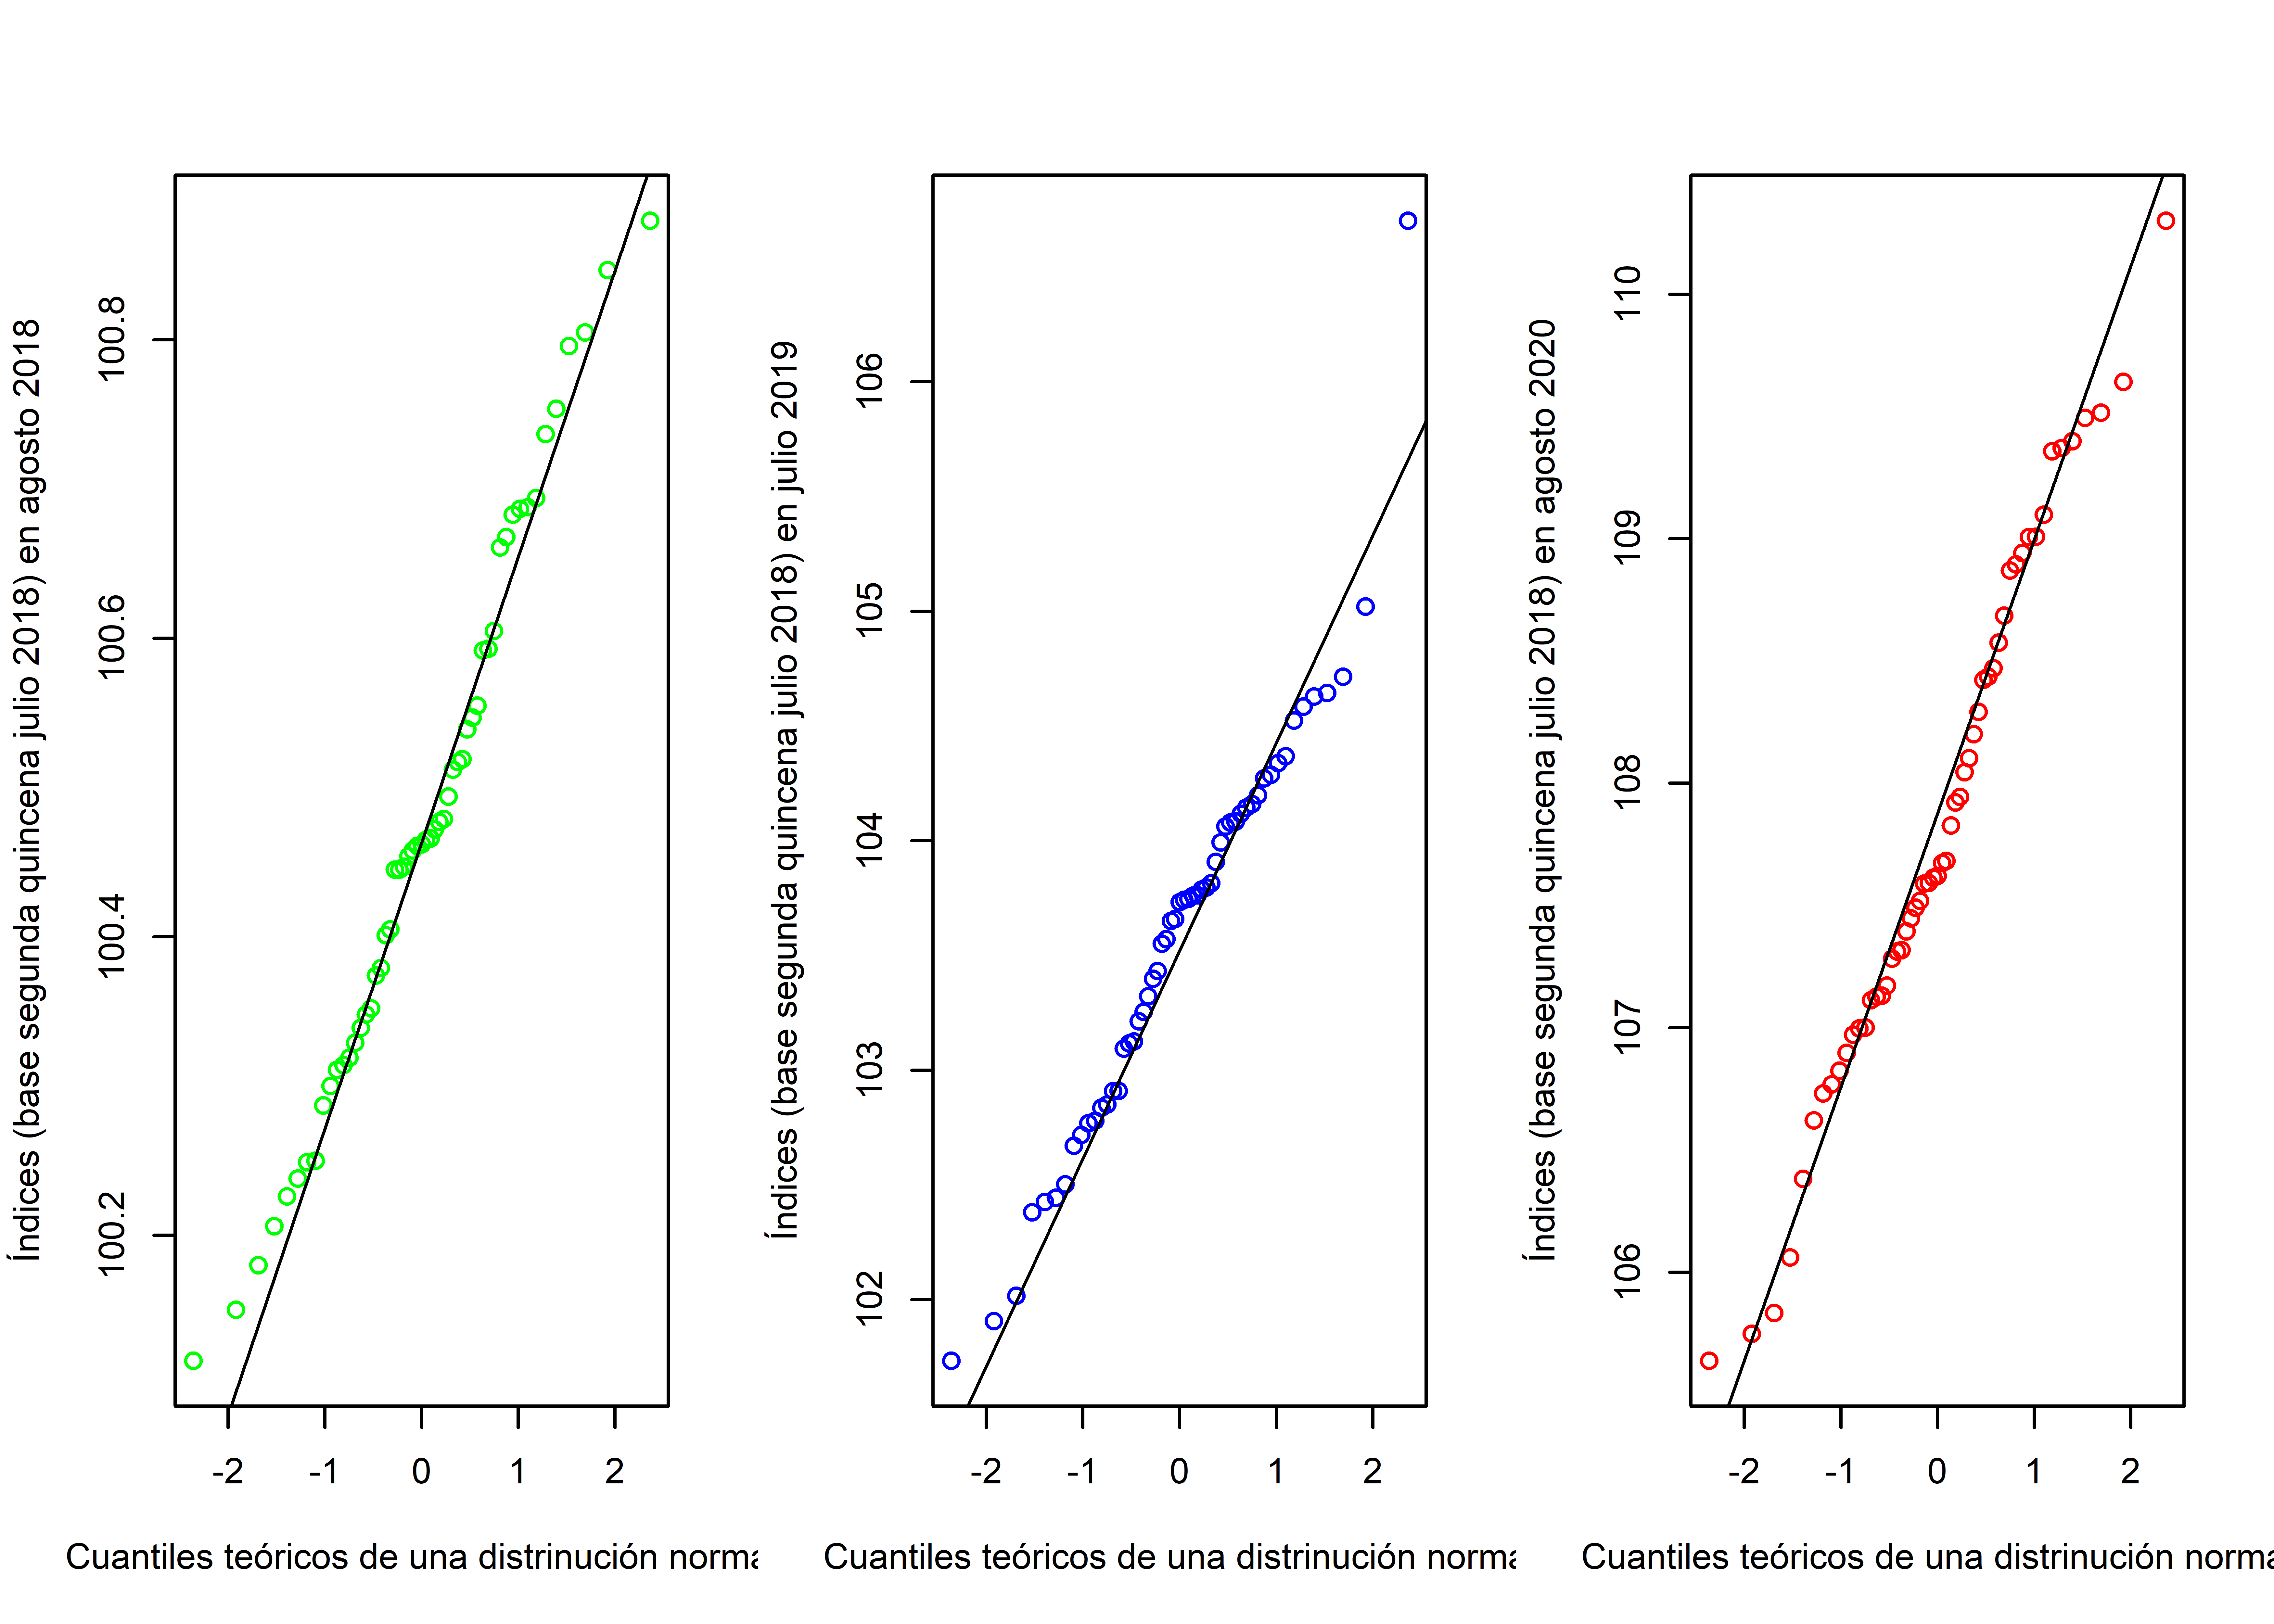
\includegraphics[scale=0.7]{Figures/normalesC2.png}
\caption{Comparativo de las gráficas QQ Normal de los  datos con los índices de las $55$ ciudades del INPC en los meses de agosto 2018 (verde), julio 2019 (azul) y agosto 2020 (rojo)}
\label{normalesC2}
\end{figure}

De acuerdo a lo anterior, para efectos de las pruebas que requieren datos con distribución normal, utilizaremos los datos del Conjunto 2 y para las pruebas que requieren que los datos no sigan una distribución normal, utilizaremos los datos del Conjunto 1.

\subsection{Prueba $t$ de student}
    
Esta prueba paramétrica se utiliza para probar si la media ($\mu$) de una muestra con distribución normal es igual a un valor especifico.

Para esta prueba se plantea como $H_{0}$ que los datos del mes de agosto 2018 tienen una $\mu$ = 100.4 y, como $H_{1}$ que estos datos tienen una $\mu$ diferente. Se utilizó la función \texttt{t.test} para realizar esta prueba. De acuerdo al resultado arrojado por la función, el valor $p =$ 0.005324, por lo tanto, se rechaza la $H_{0}$, lo cual indica que los datos del mes de agosto 2018 no tienen una media $\mu =$ 100.4. 

\subsection{Prueba de los rangos con signo de Wilcoxon}
    
Esta prueba paramétrica se utiliza para probar si la media ($\mu$) de una muestra, que se supone no sigue una distribución normal, es igual a un valor especifico. Para esta prueba se plantea como $H_{0}$ que el promedio de los datos de la ciudad de Monterrey tienen una media de $\mu =$ 98.5 y, como $H_{1}$ que en promedio estos datos no tienen esta media. Se utilizó la función \texttt{wilcox.test} para realizar esta prueba. De acuerdo al resultado arrojado por la función, el valor $p$ = 0.1779, por lo tanto, no se rechaza la $H_{0}$, lo cual indica que el promedio de los datos de la ciudad de Monterrey supone tener una $\mu =$ 98.5.
    
\subsection{Prueba $t$ de student y Wilcoxon para dos muestras}
    
Ambas pruebas se pueden utilizar para comparar la media de 2 muestras. La diferencia es que la prueba t supone que las muestras que se prueban siguen una distribución normal, mientras que para la prueba Wilcoxon se supone que no tienen este tipo de distribución los datos analizados.
    
Para la prueba de Wilcoxon se plantea como $H_{0}$ que los datos de la ciudad de Monterrey y Guadalajara tienen la misma media ($\mu_{1} - \mu_{2} = 0 $) y, como $H_{1}$ que sus medias son diferentes ($\mu_{1} - \mu_{2} \neq 0 $). De acuerdo al resultado arrojado por la función, el valor $p$ = 0.5642, por lo tanto, no se rechaza la $H_{0}$, lo cual indica que las medias de estas dos muestras, al parecer (una probabilidad del 56.42\%), son iguales. Esto significa que en el periodo de enero 2015 a agosto 2020, el INPC de Monterrey y Guadalajara fue similar. Este comportamiento lo podemos observar en la figura \ref{comparativoW}.
    
\begin{figure}
\centering
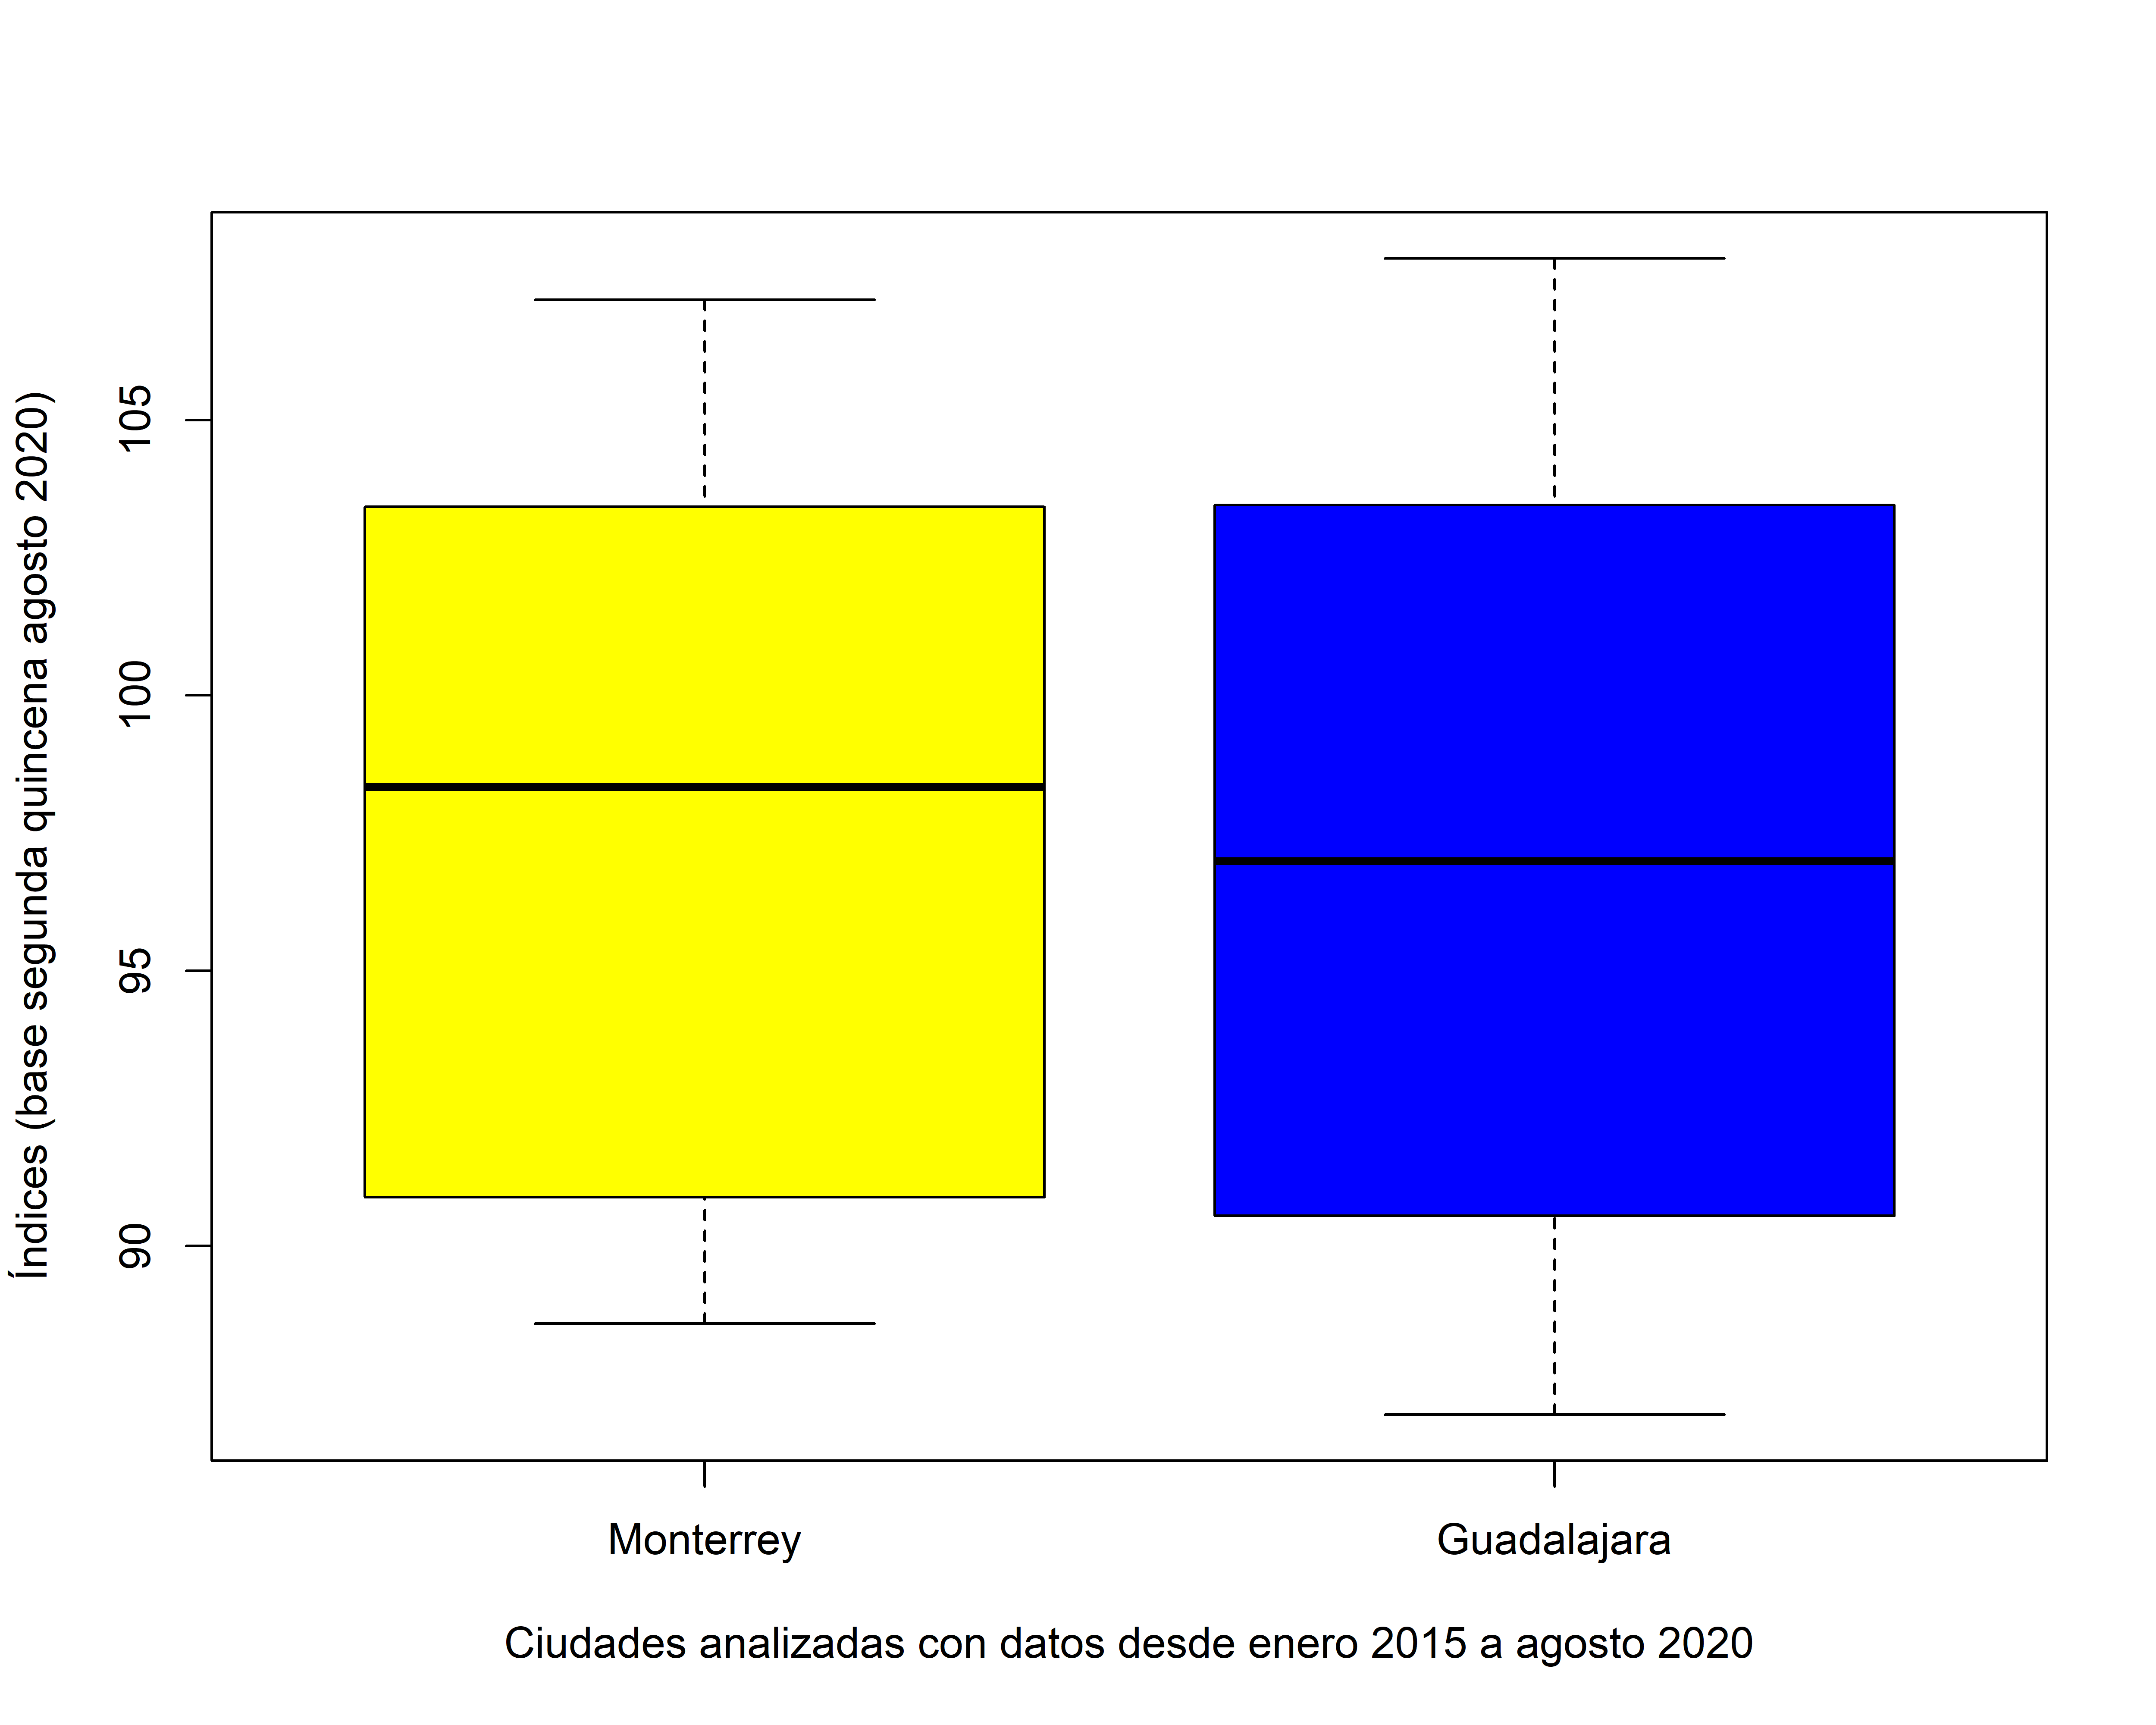
\includegraphics[scale=0.5]{Figures/comparativosW.png}
\caption{Comparativo de los diagramas de caja y bigotes con los  datos recopilados desde enero 2015 a agosto 2018 de los INPC de las ciudades de Monterrey (amarillo) y Guadalajara (azul)}
\label{comparativoW}
\end{figure}
    
Para la prueba de $t$ se plantea como $H_{0}$ que los datos de los meses de agosto de 2018 y agosto 2020 tienen la misma media y, como $H_{1}$ que sus medias son diferentes. De acuerdo al resultado arrojado por la función, el valor $p$ = 2.2$\times 10^{-16}$, por lo tanto, se rechaza la $H_{0}$, lo cual indica que, con una probabilidad muy baja, las medias de estas dos muestras son iguales. En términos del ejercicio, de acuerdo a la figura \ref{comparativosT}, el INPC promedio de las $55$ ciudades en el mes de agosto de 2018 ($\mu_{1}=$ 100.4723) fue más bajo que el promedio reportado en agosto de 2020 ($\mu_{2}=$ 107.8254), es decir, son más costosos los precios de la canasta de bienes y servicios en el mes agosto 2020 que hace 2 años.

\begin{figure}
\centering
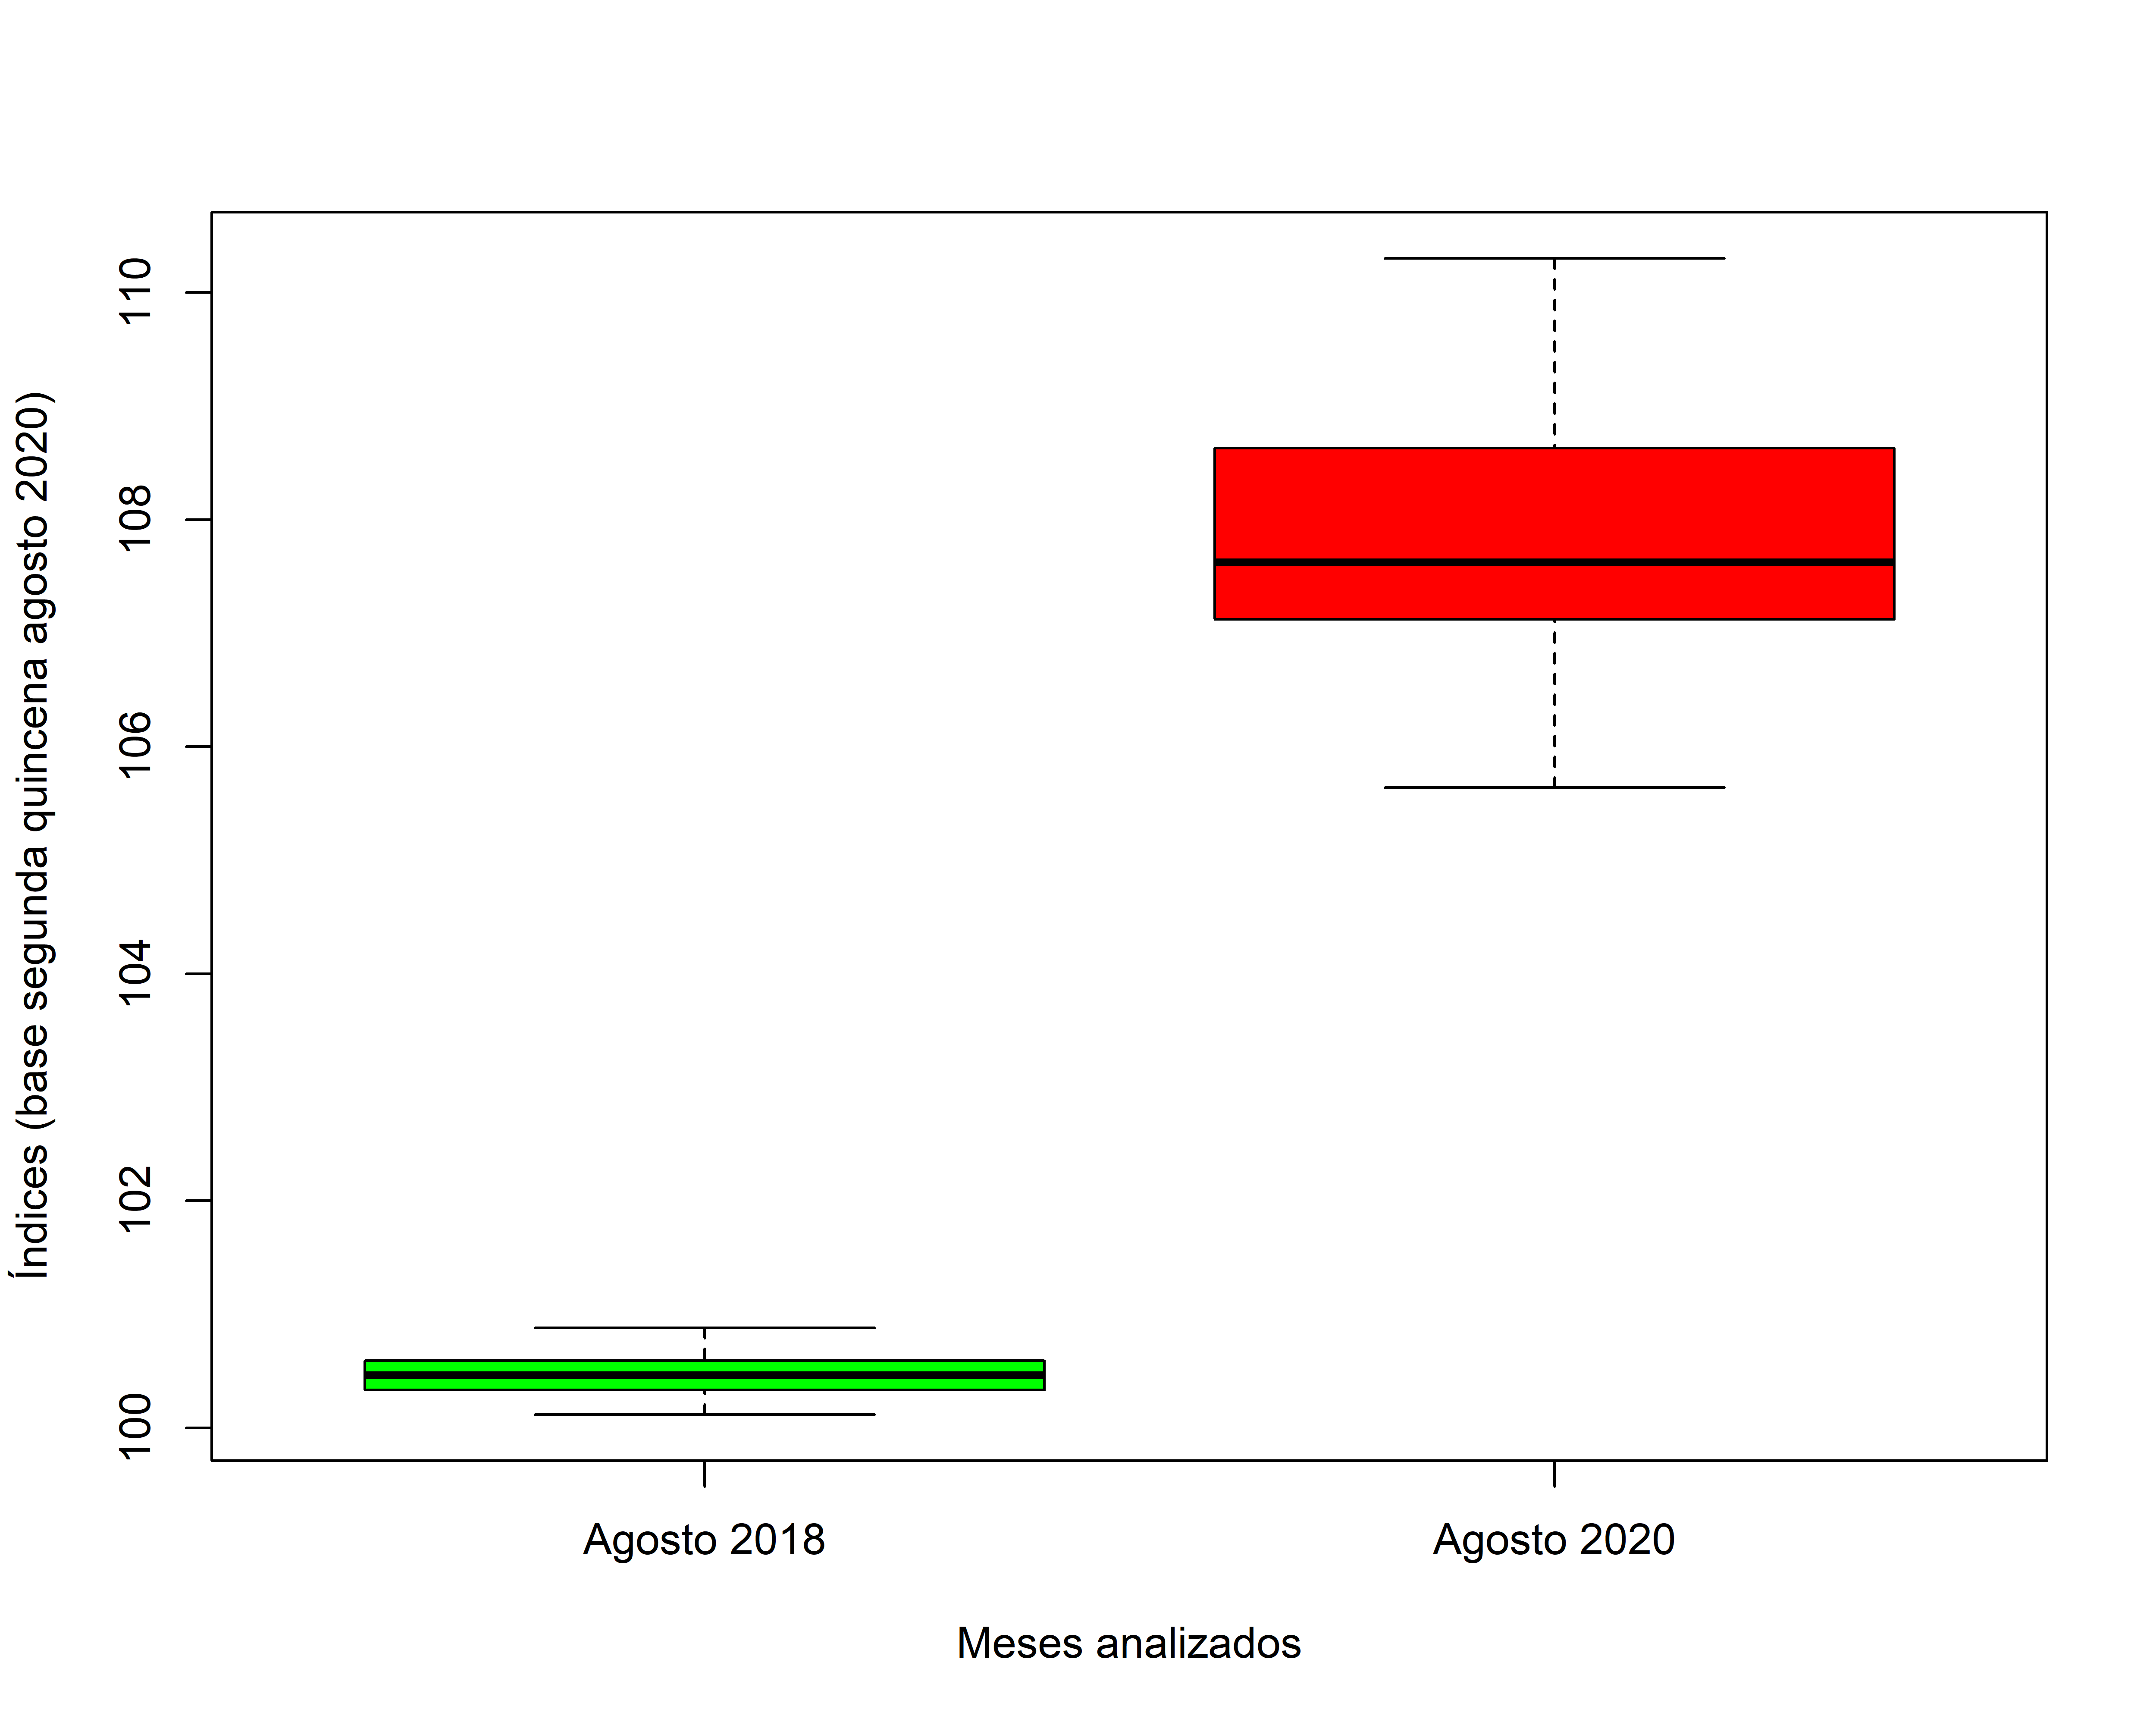
\includegraphics[scale=0.55]{Figures/comparativosT.png}
\caption{Comparativo de los diagramas de caja y bigotes con los  datos recopilados de las $55$ ciudades del INPC en los meses agosto 2018 (verde) y agosto 2020 (rojo)}
\label{comparativosT}
\end{figure}

\subsection{Prueba de Kolmogorov\textendash Smirnov}
    
Esta prueba se utiliza para comprobar si 2 muestras siguen la misma distribución. Para su desarrollo se plantea como $H_{0}$ que los datos de Cd. México y Guadalajara tienen una misma distribución y, como $H_{1}$ que estas muestras no tienen la misma distribución. Se utilizó la función \texttt{ks.test} para realizar esta prueba. De acuerdo al resultado arrojado por la función, el valor $p =$ 0.7384, por lo tanto, no se rechaza la $H_{0}$, lo cual indica que, al parecer, los datos de Cd. México y Guadalajara tienen una misma distribución.
    
\VerbatimInput{Resulpruebas/kolmogorov.txt}
    
\subsection{Prueba $F$ de Fisher}
    
Es una prueba paramétrica que se utiliza para verificar si dos muestras tienen la misma varianza. Se plantea como como $H_{0}$ que los datos de los meses de agosto 2018 con julio 2019 tienen la misma varianza y, como $H_{1}$ que estas muestras sus varianzas son diferentes. Se utilizó la función \texttt{var.test} para realizar esta prueba. De acuerdo al resultado obtenido por la función, el valor $p$ = 2.2$\times $10^{-16}$, por lo tanto, se rechaza la $H_{0}$, lo cual indica que los datos de los meses de agosto 2018 y julio 2019 no tienen la misma varianza. 
    
\VerbatimInput{Resulpruebas/fisher.txt}
    
Esta prueba también se puede usar para saber si la varianza de una muestra sigue un determinado valor, solo hay que adicionar ciertos parámetros en la función \texttt{var.test} para realizarla. Se pueden ver ejemplos en el repositorio de Freddy \cite{freddy}.
    
\subsection{Prueba $X^2$}
Esta prueba se puede utilizar para probar si dos variables categóricas son dependientes, mediante una tabla de contingencia. Para realizar esta tabla, se consideraron dos factores, ciudades y meses del año. Para las ciudades, se contemplan Monterrey y Guadalajara y se analizaran los índices de los 12 meses del año 2016. En el cuadro \ref{tablacontingencia}, se encuentra la información de los datoa a analizar.
    
\begin{table}
\centering
\caption{Tabla de contingencia para la prueba Chi$^2$}
\begin{tabular}{|l|c|c|}
\hline
         & Monterrey & Cd. México \\ \hline
 Ene 2016 & 90.779    & 88.461     \\ \hline
 Feb 2016 & 91.292    & 88.878     \\ \hline
 Mar 2016 & 91.400    & 89.077     \\ \hline
 Abr 2016 & 90.261    & 88.921     \\ \hline
 May 2016 & 90.250    & 88.946     \\ \hline
 Jun 2016 & 90.314    & 88.961     \\ \hline
 Jul 2016 & 90.505    & 89.381     \\ \hline
 Ago 2016 & 90.992    & 89.636     \\ \hline
 Sep 2016 & 91.635    & 90.216     \\ \hline
 Oct 2016 & 92.835    & 90.383     \\ \hline
 Nov 2016 & 93.108    & 90.620     \\ \hline
 Dic 2016 & 93.460    & 91.052     \\ \hline
\end{tabular}
\label{tablacontingencia}
\end{table}

Se plantea como $H_{0}$ que valores del índice alcanzado de cada ciudad es independiente del mes del año en que se encuentren y, como $H_{0}$ las variables son dependientes. Se utilizó la función \texttt{chisq.test} para realizar esta prueba. Para aceptar la $H_{0}$ se deben de cumplir dos consideraciones, que el valor $p >$ 0.05 y que el $X-Square$ sea menor al valor crítico. Para calcular este valor se utiliza la función \texttt{qchisq(0.95, n-1)}, donde 0.95 es el nivel de confianza y n-1 son los grados de libertad. Estos grados de libertad dependen de la cantidad de filas y columnas que tenga la tabla de contingencia y se calculan con la siguiente formula: ($filas-1$)$*$($columnas-1$). Para este caso, el valor crítico = 19.67514.

Al aplicar la función se obtiene que el valor $p =$ 0.2329 y un $X-Square >$ valor crítico, por lo tanto, al no cumplirse la consideración con base al $X-Square$, hay suficiente evidencia estadística para rechazar $H_{0}$, lo cual indica que las variables son dependientes, es decir, el índice de las ciudades de Monterrey y Guadalajara dependen del mes del año.

\VerbatimInput{Resulpruebas/chi.txt}
   
\subsection{Prueba de correlación}
    
Es una prueba paramétrica que se utiliza para probar si hay una relación lineal de dos variables continuas. Se pretende determinar si hay una correlación entre los índices de los de meses de julio 2019 y agosto 2020. Se plantea entonces como $H_{0}$ que los datos del mes de julio 2019 no están relacionados con el mes de de agosto 2020 y, como $H_{1}$ existe una relación entre estas variables. Se emplea la función \texttt{cor.test}. De acuerdo a los resultados arrojados por la prueba, el valor $p =$ 1.136$\times 10^{-9}$, por lo tanto, se rechaza la $H_{0}$, lo cual indica que, los datos de los meses de julio 2019 y agosto 2020 tienen alguna correlación. En la figura \ref{correlacion} se muestra el diagrama de dispersión de los datos en el que visualmente se puede observar esta correlación.
    
\VerbatimInput{Resulpruebas/correlacion.txt}

\begin{figure}
\centering
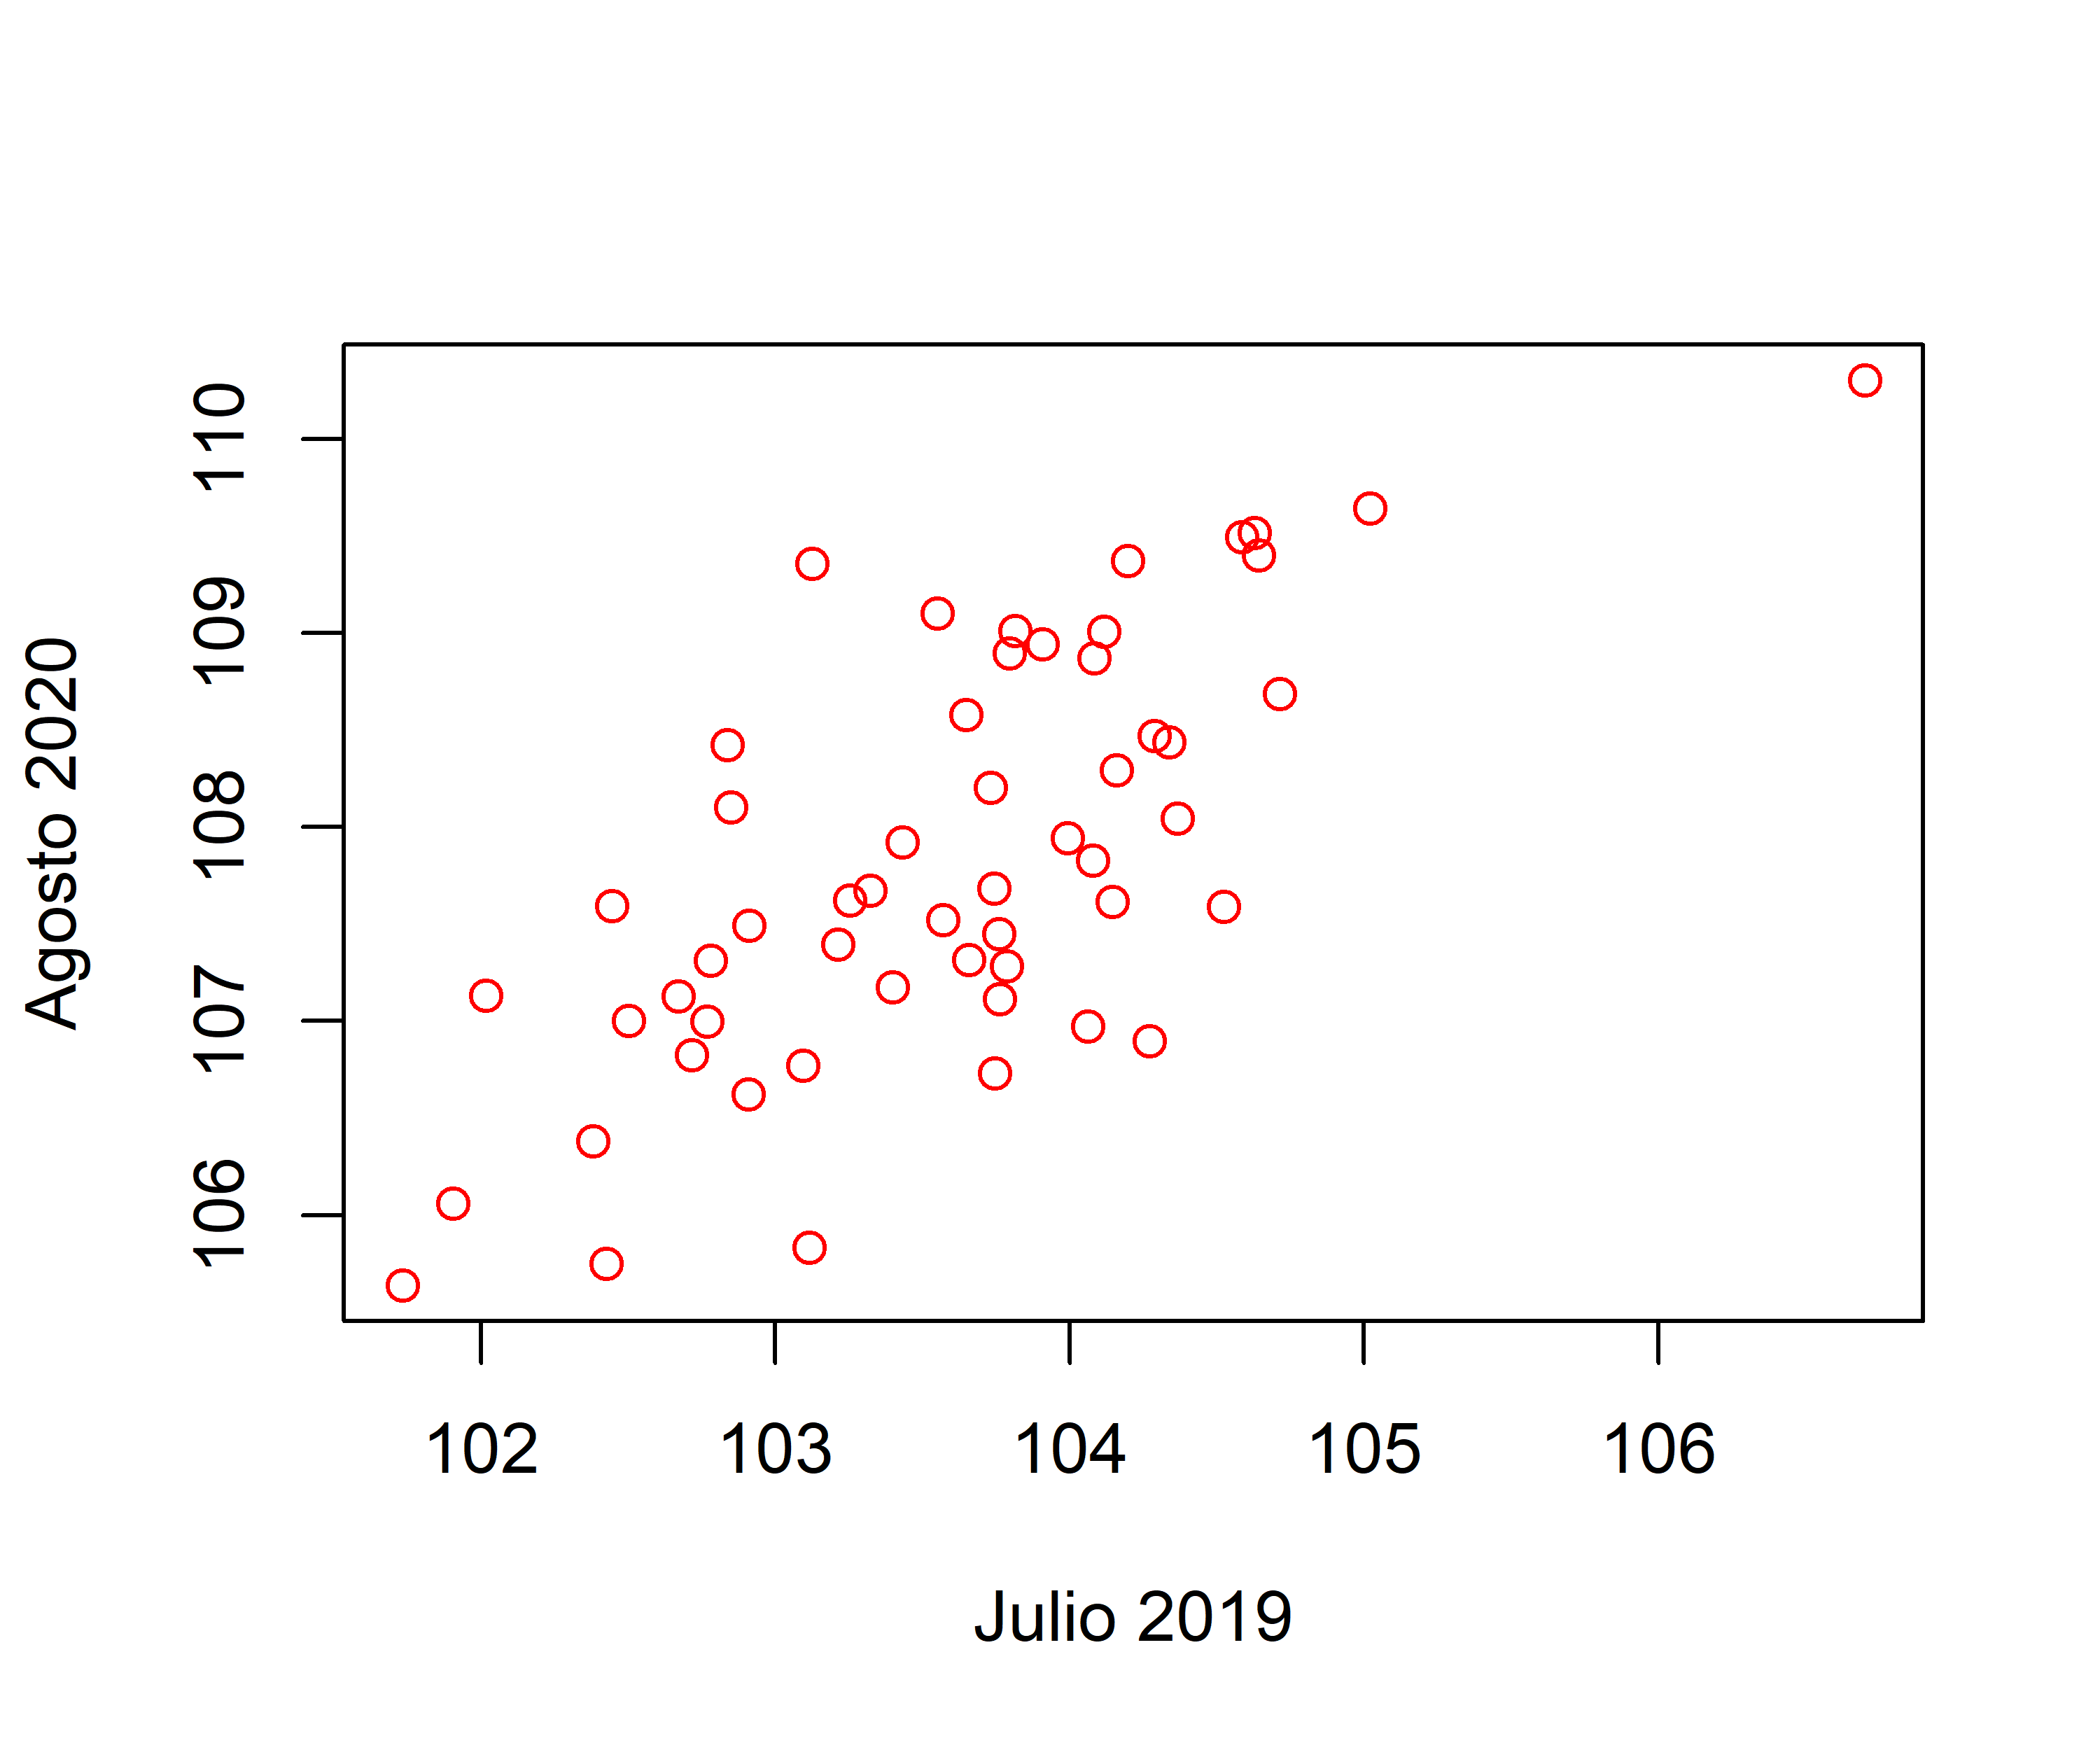
\includegraphics[scale=0.7]{Figures/correlacion.png}
\caption{Diagramas de dispersión de los índices en los meses de julio 2019 y agosto 2020}
\label{correlacion}
\end{figure}

\section{Preguntas}

A continuación, se presentan algunas de las preguntas más frecuentes para determinar que prueba estadística escoger y la interpretación de sus resultados.

\begin{itemize}
    \item Relación entre contraste de hipótesis y pruebas estadísticas
    
    Las pruebas estadísticas son técnicas que utilizan muestras representativas de una población para evaluar la evidencia que proporcionan los datos y la hipótesis es la suposición de algún fenómeno o problema la cual son comprobadas a través de las pruebas estadísticas. En estas pruebas existen dos tipos de hipótesis, nula ($H_{0}$) y la alternativa ($H_{1}$ o $H_{A}$).

    \item ¿Qué indicaría rechazar la hipótesis nula?
    
    Normalmente, la hipótesis nula ($H_{0}$) establece la igualdad entre las medias, varianzas, entre otros, por lo tanto, si se rechaza indicaría que existe alguna diferencia entre ellas.
    
    \item ¿Cómo se interpreta la salida de una prueba estadística?
    
    Al diseñar un estudio, se especifica un nivel de significación alfa ($\alpha$) que debería estar entre $0$ y $1$, lo que indica que por encima este valor $H_{0}$ no debería ser rechazada. La prueba estadística produce un número denominado valor $p$ el cual también se encuentra entre $0$ y $1$. En términos más prácticos, el valor $p$ se compara con $\alpha$, si $p < \alpha$, rechazamos $H_{0}$ y aceptamos Ha con un riesgo proporcional al valor $p$ de ser errónea. Por otro lado, si $p > \alpha$, no rechazamos $H_{0}$, pero esto no implica necesariamente que debamos aceptarla, solo que nuestro experimento y nuestra prueba estadística no han sido suficientemente ``fuertes" para producir un valor $p$ inferior a $\alpha$.

    \item ¿Cómo seleccionar el alpha?
    
    El nivel de significancia se denota con la letra griega alfa $\alpha$. No existe una evidencia científica de cuál sea el valor más adecuado. Sin embargo, el valor más empleado es 0.05, se suelen tomar valores pequeños (menores al $10\%$), esto debido a que representa el riesgo de rechazar la hipótesis nula ($H_{0}$) cuando es verdadera. En ese sentido con una buena elección de $\alpha$ se delimita muy bien cuando rechazar la $H_{0}$ lo que aumenta la probabilidad de tomar la decisión correcta.
    
    \item ¿Cuáles son los errores frecuentes de interpretación del valor $p$?
    
    La interpretación del valor $p$ conduce al rechazo o la aceptación de la hipótesis nula, específicamente el valor $p$ corresponde al menor valor de alfa ($\alpha$) que ocasiona el rechazo de la hipótesis nula ($H_{0}$). Los errores más frecuentes que se presentan son los errores tipo I y tipo II. El error tipo I se presenta cuando se rechaza la $H_{0}$ y es verdadera, mientras que el error tipo II consiste en no rechazar la $H_{0}$ cuando es falsa. De acuerdo a Walpole \cite{walpole}, en el cuadro \ref{errores} se resumen estos errores. La probabilidad de cometer esos errores se reduce aumentando el tamaño de la muestra.
    
    \begin{table}
    \centering
    \caption{Situaciones posibles al probar una hipótesis estadística}
  \begin{tabular}{|r|l|l|}
    \hline
    \multicolumn{1}{|c|}{} & \multicolumn{1}{c|}{$H_{0}$ es verdadera} & \multicolumn{1}{c|}{$H_{0}$ es falsa} \\ \hline
    No rechazar $H_{0}$    & Decisión correcta                         & Error tipo II                         \\ \hline
    Rechazar $H_{0}$       & Error tipo I                              & Decisión correcta                     \\ \hline 
    \end{tabular}
    \label{errores}
    \end{table}

    \item ¿Qué es la potencia estadística y para qué sirve?
    
    La potencia estadística o el poder del estadístico, corresponde a la capacidad que tiene una prueba de llevar al rechazo de la hipótesis nula ($H_{0}$). La potencia estadística aumenta con el valor de alfa $\alpha$, con la precisión de las medidas y el número de repeticiones, también depende del tipo de prueba estadística que se esté realizando. Este parámetro puede ser calculado antes o después de realizar el experimento.
    
    \item Ejemplos de pruebas estadísticas paramétricas y no paramétricas.
    
    Las pruebas paramétricas se emplean para datos numéricos, suelen estar basadas en las propiedades de la distribución normal para la variable dependiente. Es decir, los datos son mediciones repetidas de la misma variable, muestreado de la población realizado al azar y cuando la muestra es grande. Como ejemplo de pruebas paramétricas se tienen:
    
    \begin{itemize}
        \item La “t” de student.
        \item El coeficiente de correlación de Pearson.
        \item La regresión lineal.
        \item Análisis de varianza unidireccional (ANOVA \textit{Oneway}).
        \item Análisis de varianza factorial (ANOVA).
        \item Análisis de covarianza (ANCOVA).
        \item Estadígrafos descriptivos como la desviación estándar, la moda, la mediana y la media.
    \end{itemize}
    Por otra parte, las pruebas no paramétricas se aplican con variables nominales y ordinales, no asume un tipo específico de distribución. Ejemplos de este tipo de pruebas son:
    
    \begin{itemize}
        \item La $X^2$
        \item Coeficientes de correlación e independencia para tabulaciones cruzadas.
        \item Coeficientes de correlación por rangos ordenados Spearman y Kendll.
    \end{itemize}
    
    \item Resume LA GUIA para encontrar la prueba estadística que buscas. 
    
    \begin{itemize}
        \item Escribir claramente el objetivo de análisis.
        \item Tipo de variables.
        \item Si son muestras independientes o no.
        \item Identificar si se pueden aplicar técnicas paramétricas.
        \item Seleccionar la prueba adecuada.
        \item Realizar la prueba de hipótesis.
        \item Interpretar y graficar los resultados.
    \end{itemize}
    
    En la figura \ref{guia}, se describe el proceso de selección de una prueba estadística basado en el estudio realizado por Florez-Ruiz \cite{guia}.
    
    \begin{figure}
    \centering
    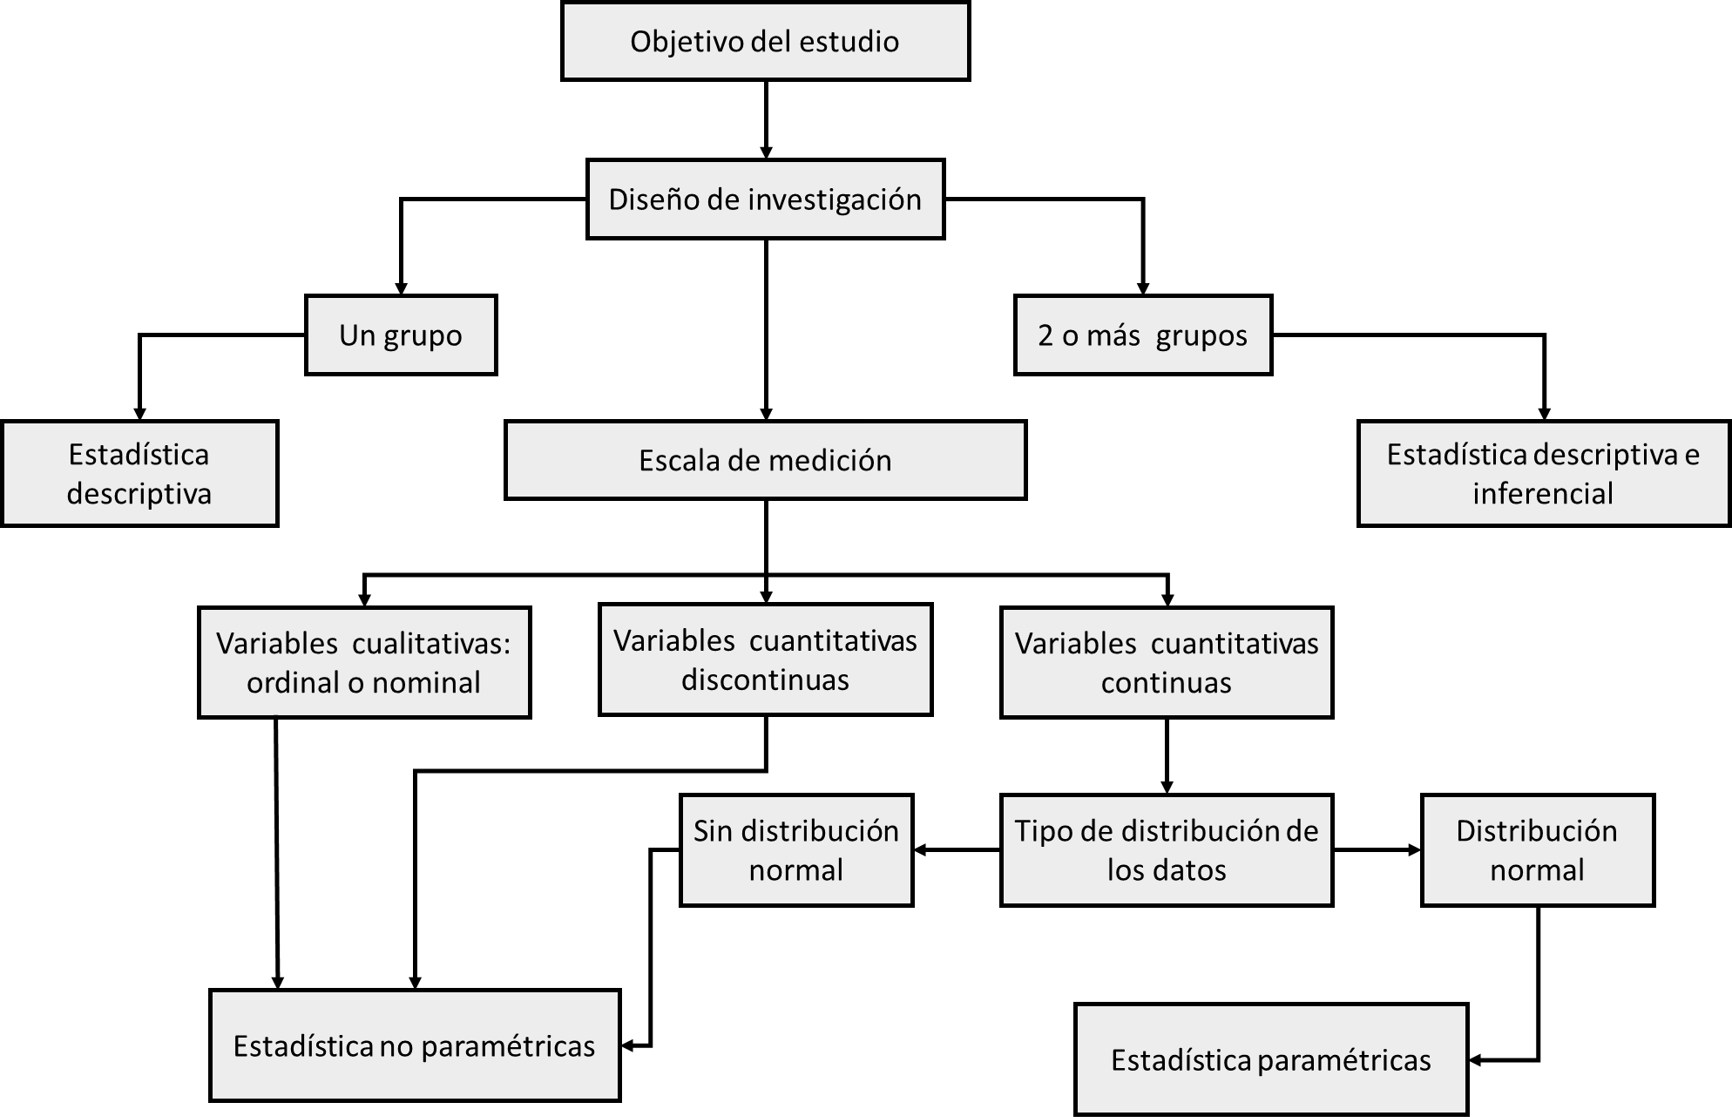
\includegraphics[scale=0.5]{Figures/resumenguia.png}
    \caption{Proceso de selección de una prueba estadística}
    \label{guia}
    \end{figure}
 
    \item ¿Cuáles son los supuestos para aplicar técnicas paramétricas?
    
    Las pruebas paramétricas están basadas en la distribución normal para la variable dependiente, y los requisitos para aplicarlas son las siguientes:
    
    \begin{itemize}
        \item Las observaciones deben ser independientes entre sí.
        \item Las poblaciones deben hacerse en poblaciones distribuidas normalmente.
        \item Estas poblaciones deben tener la misma varianza.
        \item Las variables deben haberse medido por lo menos en una escala de intervalo de manera que sea posible utilizar las operaciones aritméticas.
   \end{itemize}
\end{itemize}



\bibliography{refProbabilidad}
\bibliographystyle{plain}

\end{document}

